\documentclass[11pt]{article}

\usepackage[utf8]{inputenc}
%%\usepackage[T1]{fontenc}
\usepackage{graphicx}
\usepackage[linktocpage=true]{hyperref}

%%Page layout
\usepackage[margin=2.0cm]{geometry}
\usepackage{bookmark}

%%Figures
\usepackage{float}

\usepackage{mathpazo}

%%Font and Numbers
\renewcommand*\rmdefault{dayrom}
\usepackage[T1]{fontenc}
\normalfont
\usepackage{enumitem}

%%Packages for Referrences
\usepackage{url}
\usepackage{etoolbox}
\patchcmd{\thebibliography}{\section*{\refname}}{}{}{}
\patchcmd{\thebibliography}{\addcontentsline{toc}{section}{\refname}}{}{}{}

%%Group Comments
\usepackage{verbatim}

\begin{document}
\renewcommand{\familydefault}{\sfdefault}
\begin{titlepage}
	\newcommand{\HRule}{\rule{\linewidth}{0.5mm}}
	\begin{center}
		            
		\textsc{\LARGE Alabama Liquid Snake}\\[0.8cm]
		\textsc{\Large University of Pretoria}\\[0.5cm]
		\textsc{\large Epi-Use}\\[0.5cm]
		    
		\HRule\\[0.4cm]
		    	
		{\huge\bfseries Botic - Privacy aware chatbot}\\[0.2cm]
		    	
		{\huge System Requirements Specification}\\[0.2cm]
		
		\HRule\\[0.5cm]
		
		\textsc{Justin Grenfell} - u16028440 \\[0cm]
		\textsc{Peter Msimanga} - u13042352 \\[0cm]
		\textsc{Alicia Mulder} - u14283124 \\[0cm]
		\textsc{Kyle Gaunt} - u15330967 \\[0cm]
		\textsc{Lesego Mabe} - u15055214 \\[0cm]
		    
	\end{center}
\end{titlepage}
\tableofcontents
\newpage
\section{Introduction}
\subsection{Purpose}
The purpose of this document is to present a detailed description of Botic- the privacy aware chatbot. It will explain in good detail the purpose and the features of the system, the interfaces of the system, what the system will do, the constrainst under which it must operate and also how the system will react to user and external stimuli. This document is intended for the stakeholders, that is the COS 301 staff and lectures as well as the CS department lectures and our client EPI USE labs-- represented by Mrs. Jhani Coetzee and Mr. Tiaan Scheepers, and the developers, Alabama Liquid Snake, of the system and will be propose to all of our stakeholders for their approval.

\subsection{Background}
A crucial part of any business in today's economic climate is customer service. Those companies that are willing to go the extra mile for their customers are seen as being a cut above the rest. With superior customer service a company can not only bring in new clients, who want an experience that seems to cater to them as an individual, but also successfully retain existing clients by dealing with their issues efficiently and effectively.\par
In order to do so, there needs to be a system that can record customer feedback and act on it in as soon as possible. In the past, this has been achieved by employing a large number of people around the clock that sit and wait for queries, handle them and then send back the result.\par

While this works, it is not only inefficient (different employees may respond better or worse than others, employees may not follow protocols, mistakes may be made regularly) but financially costly as well. On top of that, when dealing accounts and queries, customers may inadvertently divulge private information that is not applicable to their case, but may leave them vulnerable should that information become public knowledge.\par

What if one central system could seamlessly record, interpret and act on the requests of multiple users 24/7 and prevent them from transmitting sensitive data unless absolutely necessary?\par

\subsection{Scope}
\textbf{Botic} is the solution! One system that can not only record user queries, but sanitize their content by filtering out any "data risks" and act on the provided information, returning the appropriate response. Trained on historical data, the system uses artificial intelligence to analyze requests and act accordingly. It scrapes all data before transmission to ensure that no sensitive information is sent to or from the client without clearance from the company's protocols first.\par

Should the system be unable to find a suitable solution, the request will be handed off to the appropriate customer representative who will then deal with the request. Once that case has been handled, the system will have learned how to deal with future requests of that type and will be able to return a response based on this learning. This will ensure a high level of efficacy for the system as a whole.\par

Botic will be the front-line for any company that provides customer service feedback facilities or services. The system will reduce the need for a large number of employees for a problem that can be solved using artificial intelligence. It will also improve efficiency and precision when dealing with issues and, due to its constantly learning nature, will become more accurate and able to handle more complex situations as time goes on.

\subsection{UML Domain Model}

\begin{figure}[H]
	\centering
	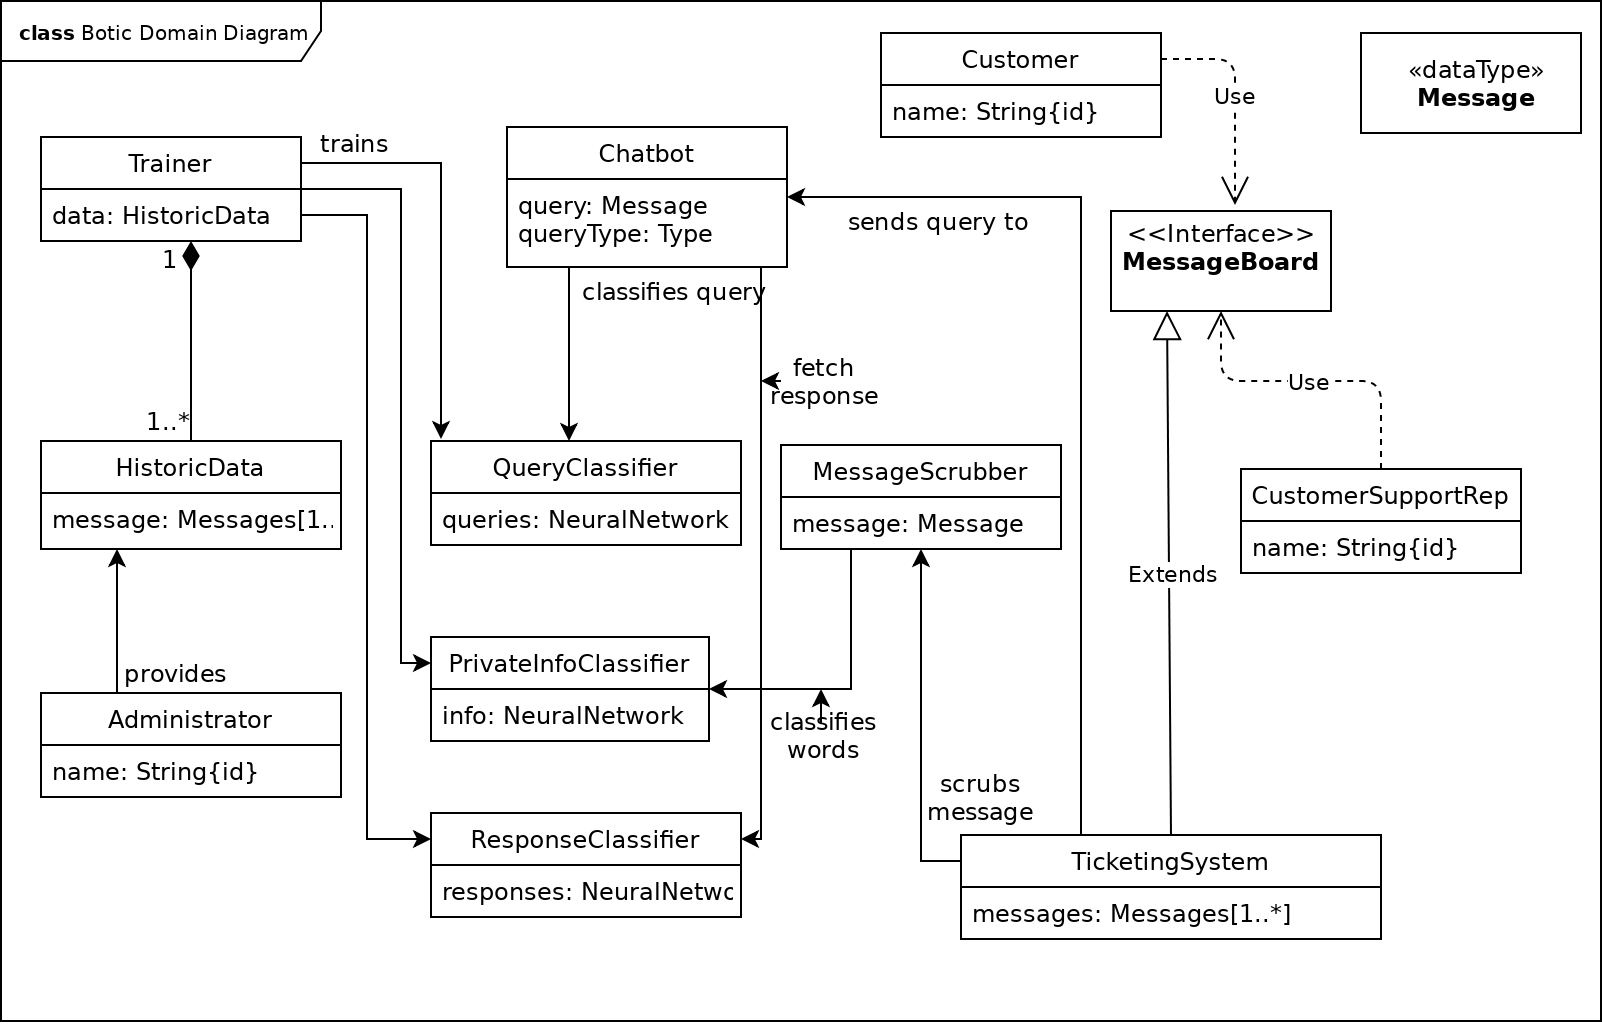
\includegraphics[width=1.0\textwidth]{../../images/Botic_Domain_Diagram.png}
	\caption{UML Domain Model of the Botic System}
\end{figure}

\subsection{Definitions, acronyms, and abbreviations}

\begin{tabular}{ |p{2cm}|p{14.7cm}| }
	\hline
	Chatbot              & A program that is designed to simulate a conversation as if it were a human, in order to assist one who queries with some task or inquiry. In the context of this project, the chatbot will be used to assit customers in a ticket system (customer service system).                                                                                                                                                     \\
	\hline
	AI                   & Artificial Intelligence;  this refers to programmed intelligence, or rather, intelligence that is demostrated by computers usually to mimick human intelligence in some specific area or even in general terms.                                                                                                                                                                                                          \\
	\hline
	Historic Data        & Data that is collected and stored over some considerable period of it time, especially, in the context of this project, with the purpose of being used to train a chatbot.                                                                                                                                                                                                                                               \\
	\hline
	POPI Act             & Protection of Personal Information Act; an South African piece of legislature aimed at protecting the right of its citizens to privacy, especially in the Internet and its periphery. It aims to "provide for the rights of persons regarding unsolicited electronic communications and automated decision making; to regulate the flow of personal information access the borders of the Republic."\cite{Legislature:1} \\
	\hline
	Ticket System        & An online platform, used by a business, made for processing customer queries and issues on products, services and the like.                                                                                                                                                                                                                                                                                              \\
	\hline
	Personal Information & Sensative and identifying information; the likes of which permission should be asked before sharing or processing.                                                                                                                                                                                                                                                                                                       \\
	\hline
	CS                   & Computer Science, as in the academic discipline of Computer Science.                                                                                                                                                                                                                                                                                                                                                     \\
	\hline
	Scrub                & Detect private information and highlight it according to severity.                                                                                                                                                                                                                                                                                                                                                       \\
	\hline
	SPA                  & Single Page Application; a web application that dynamically changes a signle page to display all of its contents.                                                                                                                                                                                                                                                                                                        \\
	\hline
	Heroku               & Deployment platform.                                                                                                                                                                                                                                                                                                                                                                                                     \\
	\hline
	Docker               & Containerization platform*.                                                                                                                                                                                                                                                                                                                                                                                              \\
	\hline
	Auth0		    &Authorization server; third party software/service; provides authorization and authentication as a service.*
\\
	\hline
\end{tabular}

\subsection{References}
\bibliographystyle{IEEEtran}
\bibliography{references}
%%IEEE. IEEE Std 830-1998 IEEE Recommended Practice for Software Requirements Specifications. IEEE Computer Society, 1998
%%http://www.cse.msu.edu/~chengb/RE-491/Papers/SRSExample-webapp.doc
%%TripleParity docs

\subsection{Overview of Document}
The next chapter, the Overall Description section, of this document gives an overview of the functionality of the project. It describes the 'informal' requirements and is used to establish a context for technical requirements specification in the next chapter.\par
The third chapter, the Requirement Specification section, of this document is written especially for the developers and describes in terns the details of the functionality of the product.\par
Both sections of the document describe the same software product in its entirety, but are intended for different audiences and thus use different languages, but seeing as virtually everyone reading this document has a CS background, the main focus ought to be the third section and it is given priority as a result.\par
This document is structured according to the IEEE 830-1998 SRS Standard\cite{Standard:1}, as recommended by:\cite{Book:1}.

\section{Overall Description}
\subsection{Product Perspective}
 
This system was originally meant to be used in an already existing customer support ticketing system, or ticket system in short. This is to say that the ticketbot- or rather, chatbot, was meant to interface with the ticket system and also be trained with the ticket system's historic data without the risk of exposing customer personal information.\par

This is system is meant to process a ticket system's messages or tickets, let the users know if they are exposing personal information, and respond intelligently to the messages otherwise divert the queries to a client representative if no sufficient response can be found.\par

However, for the purposes of this project, we will use a simple SPA to mimick the ticketing system.

\subsubsection{System Interfaces}

The ticket system interfaces with the message scrubber component by communicating to through the message scrubber's API endpoint. The ticket system sends individual words to the message scrubber which returns the severity of word-- the severity is meant to indicate the critical nature of the information revealed e.g. a password can be given the highest severity. This is done whilst the user is typing their message, and the words are highlighted accordingly in their parent field.\par

The ticket system also interfaces with the chatbot component by communicating through its API endpoint as well. This is when the ticket system sends scrubbed information to the chatbot to gather a response. Once a call is made, the ticket system is sent a reponse through the same API endpoint it called.

\subsubsection{User Interfaces}

The user interface, which is ultimately the chatbot ticket interface, is meant to be a SPA-- Single Page Application. This should be made available online in a manner that supports all major web browsers.

%%Discuss following Google's Material Design with the group

\subsubsection{Hardware Interfaces}

Each subsystem will be containerized into a Docker container, which in and of themselves use Linux 64-bit architecture. 
Ports will be mapped to port 80; this is the standard port for API's and is the port that is exposed on our deployment platform, Heroku.
%%Place the Portmapping Diagram Here, and the Docker container one as well

%%\subsubsection{Software Interfaces}
%%Include snapshots of the packages used in the frontend's packages.json, and go on like that with each subsystem, including
%%specifying how all those subsystems interacted with each other.

%%\subsubsection{Communications Interfaces}
%% SSL, HTTP, et cetera

%%\subsubsection{Memory Constraints} characteristics and limits on primary and secondary memory
%%\subsubsection{Operations} mention backup and recovery operations et cetera
%%\subsubsection{Site Adaptation Requirements} mention dev and production modes

\subsection{Product Functions}%%Functional Requirements;

The Botic system consists of the frontend, AI backend which includes the chatbot API, message scrubber API, the classifier API and their neural networks. The frontend is a Single Page Application which houses the main user interface of the system. The Chatbot API is responsible for recieving messages and returning responses.\par

The Message Scrubber API checks whether or not information provided to it is private and if so, determines the severity of it. The neural networks are trained using Machine Learning and provide the system with its intelligences-privacy classification, responses to queries and queries classification.

%%Use a component diagram to illustrate this point
%%Below this you should have use case diagrams and block diagrams for the architecture
\subsubsection{Authentication}

This subsystem is to be responsible for the authentication and the authorization of customers and customer representatives. This involves the creation and update of user profiles of the mentioned roles. Auth0 will be used as an Authorization server and will be configured to make us of the OAuth 2.0 authorization framework in order to provide us with enough flexibility to create different grants/permissions to easily authorize different users for different activities in the system.

\begin{figure}[H]
	\centering
	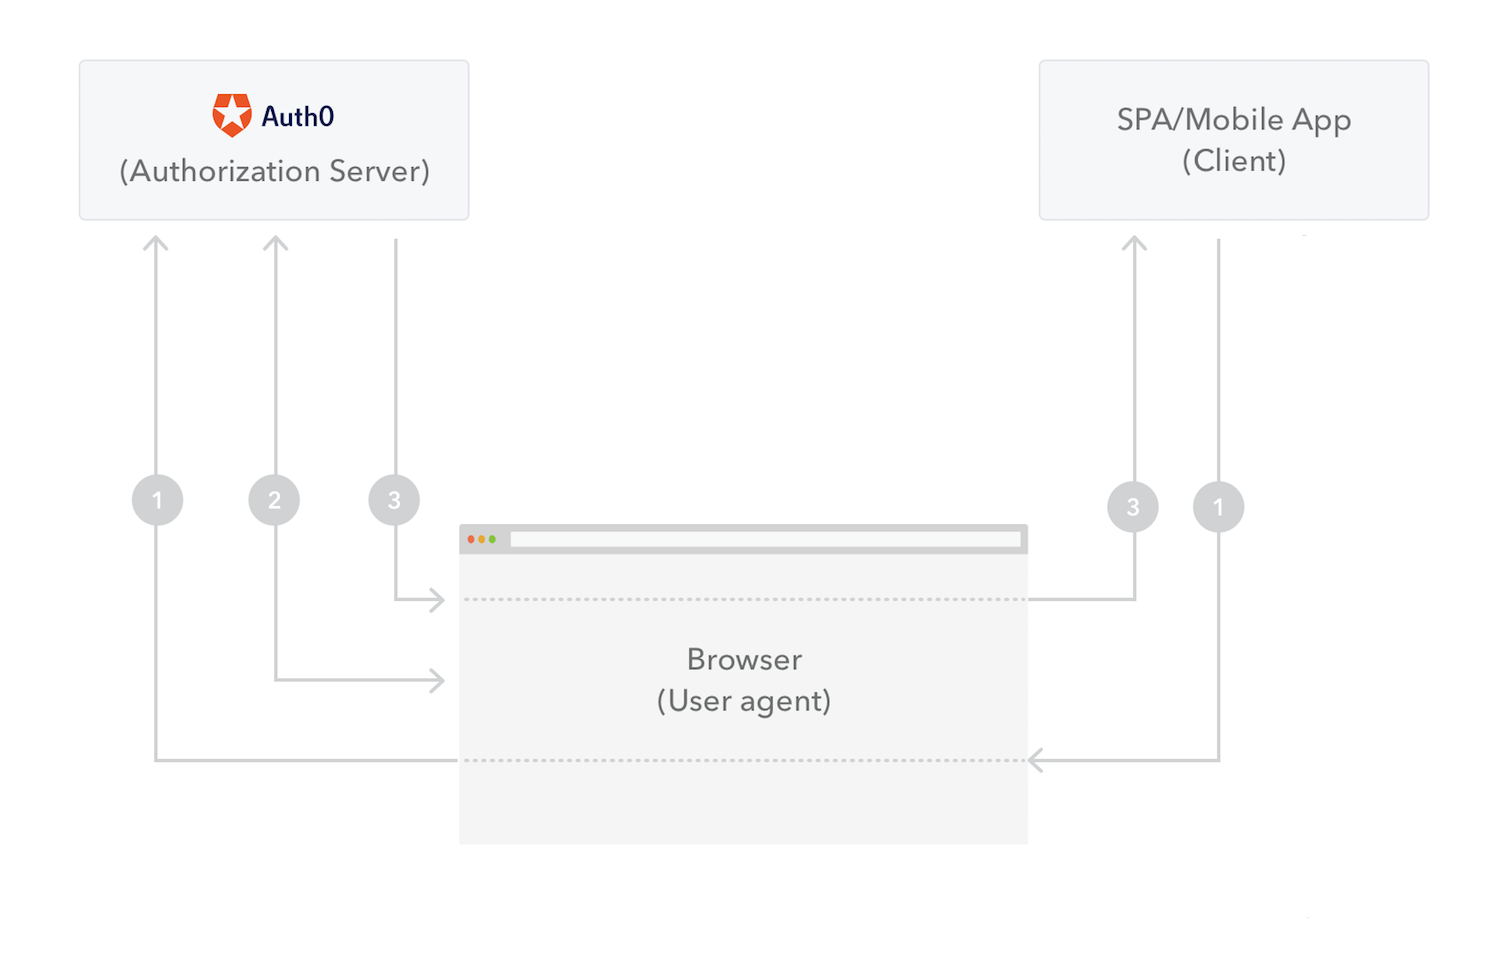
\includegraphics[width=1.0\textwidth]{../../images/implicit-grant.png}
	\caption{Auth0 Solution Diagram\cite{Website:1}}
\end{figure}

\begin{enumerate}
	\item The frontend initiates the flow when the user clicks on the sign in button and redirects the browser to the Auth0 			/authroze endpoint so that the user can be authenticated.
	\item Auth0 then authenticates the user. If the user is using one of the supported social logins, they will be shown a 			consent page where there are permissions, which will be given to our system- Botic, that a listed and they would have to 		give their consent for Botic, through Auth0, to use.
	\item Auth0 then redirects to Botic with an Access Token in the hash fragment of the URI, which the authentication 			module consumes. The happens because Auth0 calls an endpoint on the Botic fronend which processes the token from the 	URI. Botic can now extract the token, and the user is logged in.\cite{Website:1}
\end{enumerate}

\subsubsection{Information Scraper}

\begin{figure}[H]
	\centering
	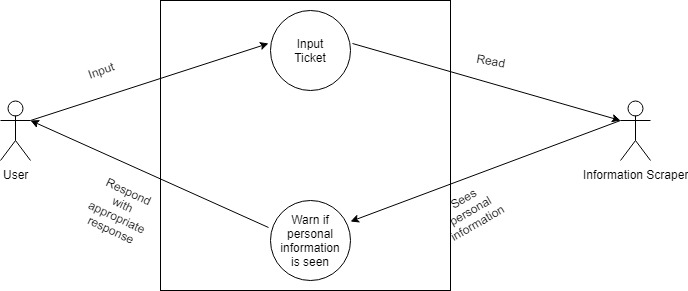
\includegraphics[width=1.0\textwidth]{../../images/Information_Scraper_UCD.jpg}
	\caption{UML Use Case of the Information Scraper}
\end{figure}

The Information Scraper, or Message Scrubber, is a subsystem that is responsible for identifying personally identifying information as the user types in their query. It uses the PrivateInfoClassifier to classify words given to it and to produce a severity index. It is called by an interface that is implemented as an Angular service in the Botic frontend. The API itself is implemented in Python and served using gunicorn. It is containerized using Docker to make it more portable, and also to make it possible to run it and other subsystems in the same infrastructure without much difficulty.

\subsubsection{Chatbot/Ticketbot}

\begin{figure}[H]
	\centering
	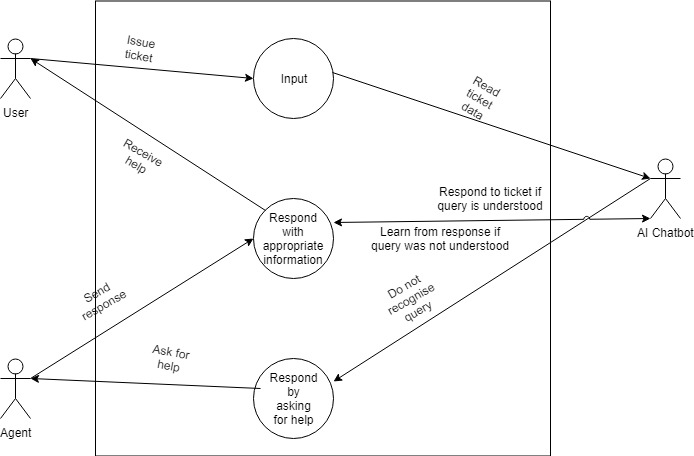
\includegraphics[width=1.0\textwidth]{../../images/AI_Chatbot_UCD.jpg}
	\caption{UML Use Case of the Chatbot}
\end{figure}

The Chatbot or 'Ticketbot' is the subsystem that is responsible for taking in customer queries and answering those queries. The Chatbot consults a QueryClassifier with a query to classify it i.e. whether it is a password, configuration, or other query for example. The classification and the query are then used to find the best response for the query using a neural network of responses, which was initially trained using historical data. The Chatbot is implemented using Nodejs and it is also containerized, for the same reasons as the previous subsystem.

\subsubsection{AI Training}

\begin{figure}[H]
	\centering
	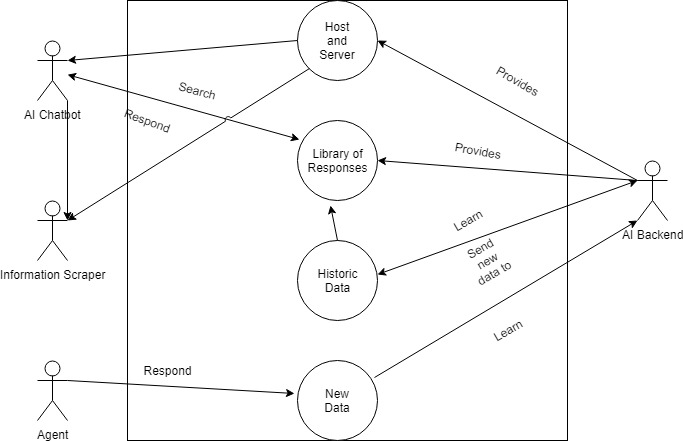
\includegraphics[width=1.0\textwidth]{../../images/AI_Backend_UCD.jpg}
	\caption{UML Use Case of the AI Backend}
\end{figure}

The AI Training subsystem is responsible for training the PrivateInfoClassifier, the QueryClassifier and the Responses neural networks. This is done using historic data which belongs to the ticketing system.

\subsubsection{Database Manager}

This subsystem is responsible for managing persistance in the system. It is called when data needs to be stored, updated, and deleted. Each endpoint will require that the subsystem calling it, identify itself. We intend to have this API secured using JSON Web Tokens. It will be implemented using Java, which when correctly uses, tends to outperform Nodejs is speed\cite{Website:2}  and is a much more rebust language than that of NodeJs's JavaScript\cite{Website:2}. This language choice is also made with consideration to the data analytics what will come about when analyzing and processing logs and their data.
%%It's also much easier to translate knowledge we learnt in COS226 for concurrency usage, than learn to do it with another
%%language due to time constraints. All team members know how to implement concurrency using Java.
%%Also, in terms of maintainability, using Java over time will result in a much faster and robust system.

\subsection{User Characteristics}

\subsubsection{Customer}
The customer will be submitting information to the system in order to deal with account related queries and, in doing so, may unintentionally submit private/sensitive information that could lead to a breach of confidentiality. Any information sent through by the customer will be sanitized by the system and cleaned up before it is transmitted.

\subsubsection{Customer Support Representative}
This user will be notified when the automated system is unable to interpret the customer's request and said request will be forwarded. The user will have the ability to respond with the result, whereby the system will sanitize the data once more and send it through to the customer.

%%\subsection{Constraints}
%%\subsection{Assumptions and Dependencies}
\section{Specific Requirements}
%\subsection{External Interfaces}

\subsection{Functional Requirements} %used to be \subsection{Function}

\subsubsection{Authentication}
\begin{enumerate}[label=R1.\arabic*.]
	\item The system must be able to authenticate users and authorize them to access system features.
	\begin{enumerate}[label*=\arabic*.]
		\item The system must be able to authenticate users using Auth0 and recieve an access token.
		\item The system must be able to identify a users' Email after being authenticated.
		\item The system must be able to check access tokens to see if they have correct permissions.
	\end{enumerate}
	\item The system must be able to deny users who haven't been authenticated to access system features
	\begin{enumerate}[label*=\arabic*.]
		\item The system must be able to check login status and access tokens.
		\item The system must be able to check permissions within access tokens.
	\end{enumerate}
	\item The system must be able to allow new users to register for user profiles for authentication.
	\item The system must be able to allow users to update their password.
\end{enumerate}
%%\subsubsection{UI}

\subsubsection{Information Scraper}
\begin{enumerate}[label=R2.\arabic*.]
	\item The system must be able to identify personally identifying information.
	\begin{enumerate}[label*=\arabic*.]
		\item The system must be able to read in strings to identify personally identifying information.
		\item The system must be able to use a neural network to identify personally identifying information.
		\item The system must be able to attach a severity to the personally identifying information.
	\end{enumerate}
	\item The system must be able to warn a user if they have entered identifying information.
	\begin{enumerate}[label*=\arabic*.]
		\item The system must be able to highlight personally identifying information according to severity index.
		\item The system must be able to prevent the user from sending personally identifying information.
	\end{enumerate}
\end{enumerate}

\subsubsection{Chatbot/Ticketbot}
\begin{enumerate}[label=R3.\arabic*.]
	\item The system must be able to process user queries to provide an appropriate response.
	\begin{enumerate}[label*=\arabic*.]
		\item The system must be able to allow users to send a message to the chatbot.
		\item The system must be able to use the QueryClassifier to to classify the user query.
	\end{enumerate}
	\item The system must be able to attempt to answer processed user queries/tickets.
	      \begin{enumerate}[label*=\arabic*.]
	      	\item The system must be able to use the classification of the query to obtain a response index.
		\item The system must be able to send the query to a human if it cannot obtain a response index.
		\item The system must be able to obtain a response using a response index from the Database Manager
	      \end{enumerate}
	\item The system must be able to use a text recognition API to understand the query.
\end{enumerate}

\subsubsection{AI Training}
\begin{enumerate}[label=R4.\arabic*.]
	%\item The system must host and server the AI Chatbot and Scraper respectively
	%\item The system must provide the library of responses that the AI has at its disposal.
	\item The system must be able to train on new and historic information to learn how to classify queries
	\item The system must be able to train on new and historic information to learn how to classify personally identifying information.
\end{enumerate}

\subsubsection{Database Manager}
\begin{enumerate}[label=R5.\arabic*.]
	\item The system must allow other subsystems to persist information.
	\begin{enumerate}[label*=\arabic*.]
		\item The system must store information into the system's database.
	\end{enumerate}
	\item The system must allow other subsystems to update information.
	\begin{enumerate}[label*=\arabic*.]
		\item The system must edit information in the system's database.
	\end{enumerate}
	\item The system allow other subsystem to delete information.
	\begin{enumerate}[label*=\arabic*.]
		\item The system must delete information in the system's database.
	\end{enumerate}
\end{enumerate}

%\subsection{Performance Requirements}
%\subsection{Design Constraints}
%\subsubsection{Standards Compliance}
\subsection{Software System Attributes}%%Non-Functional Requirements (limited to 6)

The non-functional requirements below will be listed by priority.

\subsubsection{Availability}
\begin{enumerate}
	\item The system has to have high availability to handle customer queries and issues since it is meant to augment a customer support system, i.e. a ticket system.
	\item The system should be available at least 99 percent of the time, not considering network errors.
\end{enumerate}

%%\subsubsection{Reliability}

\subsubsection{Performance}
\begin{enumerate}
	\item The system must answer queries as quickly and accurately as it can or divert the query to the relevant customer support specialist in good time. 
\end{enumerate}

\subsubsection{Scalability}
\begin{enumerate}
	\item The system should be able to scale appropriately to accommodate additional/growing customer queries, especially during peak work hours; it would be useful if the resources scaled down as well during “off peak” hours.
	\item We have chosen to deploy our system to Docker, it is used in part to allow for efficient and easy scaling. More resources can be allocated to our system dynamically - on demand.
\end{enumerate}

\subsubsection{Maintainability}
\begin{enumerate}
	\item The system structure will be modular to adhere to the concept of low coupling and high cohesion. This would help to make it maintainable since updated systems result in localized changes instead of changes everywhere throughout the system.
	\item We will create a coding standards document which we will also adhere to throughout the system in order to increase readability.
\end{enumerate}

\subsubsection{Security}
\begin{enumerate}
	\item This pertains to ensuring the [authentication=appropriate word] of customers, to make sure that responses are sent to the correct users.
	\item A log-in system would have to be implemented and private customer information would have to be secured i.e information that would used for authentication purposes like E-mail addresses.
	\item We will be using OAuth for authentication purposes.
\end{enumerate}

%%\subsubsection{Portability}
\subsection{Organizing the Specific Requirements}

%%\subsubsection{System Mode}
%%\subsubsection{User Class}
%%\subsubsection{Objects}
%%\subsubsection{Feature}
%%\subsubsection{Stimulus}
%%\subsubsection{Response}
%%\subsubsection{Functional Hierarchy}

\subsubsection{Traceability Matrix}
\begin{center}
	\begin{tabular}{||c | c | c | c ||} 
		\hline
		     & Information Scraper & AI Chatbot & AI Backend \\
		\hline\hline
		R1   & X                   &            &            \\
		\hline
		R2   & X                   &            &            \\
		\hline
		R3   & X                   &            &            \\
		\hline
		R4   & X                   &            &            \\
		\hline
		R5   &                     & X          &            \\
		\hline
		R6   &                     & X          &            \\
		\hline
		R6.1 &                     & X          &            \\
		\hline
		R6.2 &                     & X          &            \\
		\hline
		R6.3 &                     & X          &            \\
		\hline
		R7   &                     & X          &            \\
		\hline
		R8   &                     & X          &            \\
		\hline
		R9   &                     &            & X          \\
		\hline
		R10  &                     &            & X          \\
		\hline
		R11  &                     &            & X          \\
		\hline
		R12  &                     &            & X          \\
		\hline
		
	\end{tabular}
\end{center}

%%\subsection{Additional Comments}
%%\section{Support Information}
%%\subsection{Table of Contents and Index}
%%\subsection{Appendixes}

\section{Architectural Design}

\subsection{System Type}

Our system type is an interactive system, as it is focused on the customer's interaction with the Chatbot. This means that the interaction begins and ends with the customer. The N-tier architecture is useful for the design of interactive systems. This architecture is breaks the system down to a number of relatively independent and loosely coupled layers.\cite{Book:1}

\subsection{Architectural Style}

We will be using a 3-tier architectural style for the first level of granularity as a result. This architectural style is in line with making sure that the entire system has prioritizes availability. The relevantly independent and loosely coupled layers makes the testing and the development of the system less couplicated. As a result, maintanence and further updates of the system benefit as well.The 3 layers themselves will be the frontend, AI (artificial intelligence) layer, and then the Data persistence layer or database layer in short.\par

The first layer, follows the MVC architecture, the Model View Controller architecture. We will be using the Angular framework, as our client requires. Here, there is a controller for each view, and certain controller types, called services which we will use to interface with our AI layer components i.e. the Chatbot, and the Message Scrubber.\par

The second layer holds the Message Scrubber, as well as the Chatbot. The final layer contains the database as well as the Database Manager.

\begin{figure}[H]
	\centering
	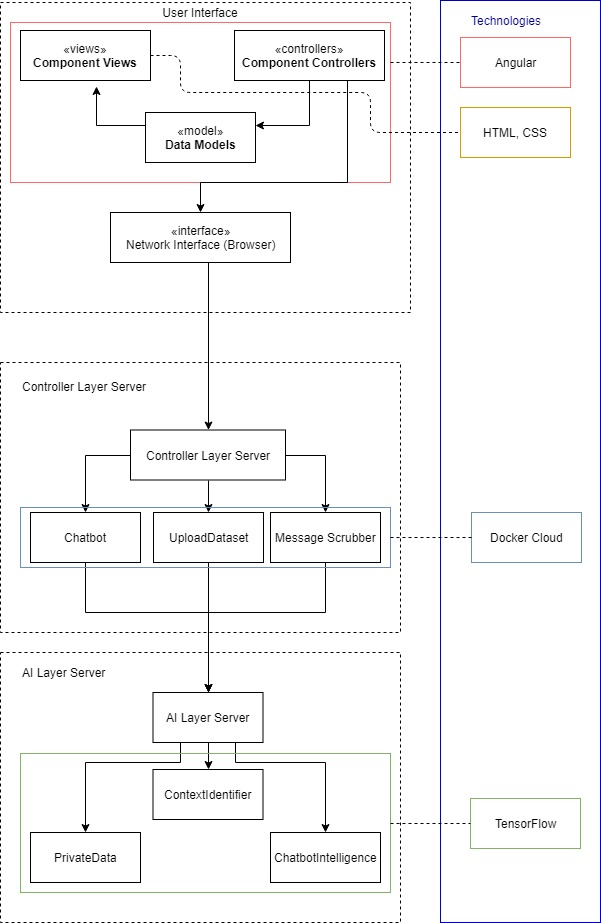
\includegraphics[width=0.5\textwidth]{../../images/Botic_Simplified_Architectural_Design.jpg}
	\caption{3-Tier Architectural Diagram}
\end{figure}

\end{document}